\documentclass{article}
\include{graphicx}
\begin{document}
\title{Supplement to ``Rapid, accurate peptide identification''}

\author{Chris Y. Park, Aaron A. Klammer, Lukas K\"{a}ll, Michael J. MacCoss
and William S. Noble}

\maketitle

\section{Sp and Xcorr comparisoin}
\begin{figure*}
  \centering
  \begin{tabular}{cc}
    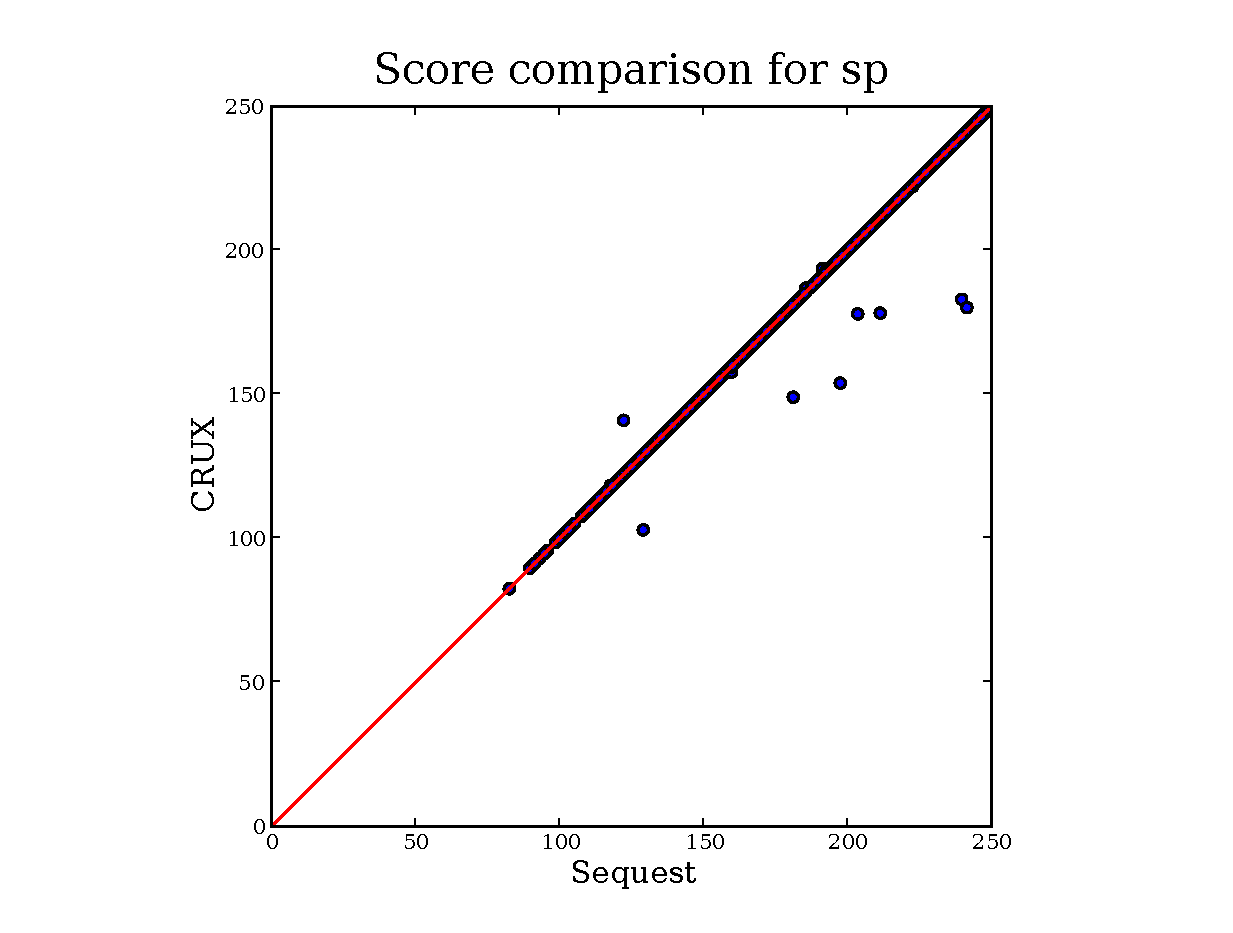
\includegraphics[width=2.5in]{../../results/paper-figure/second-score/fig-2-random-sp.eps} &
    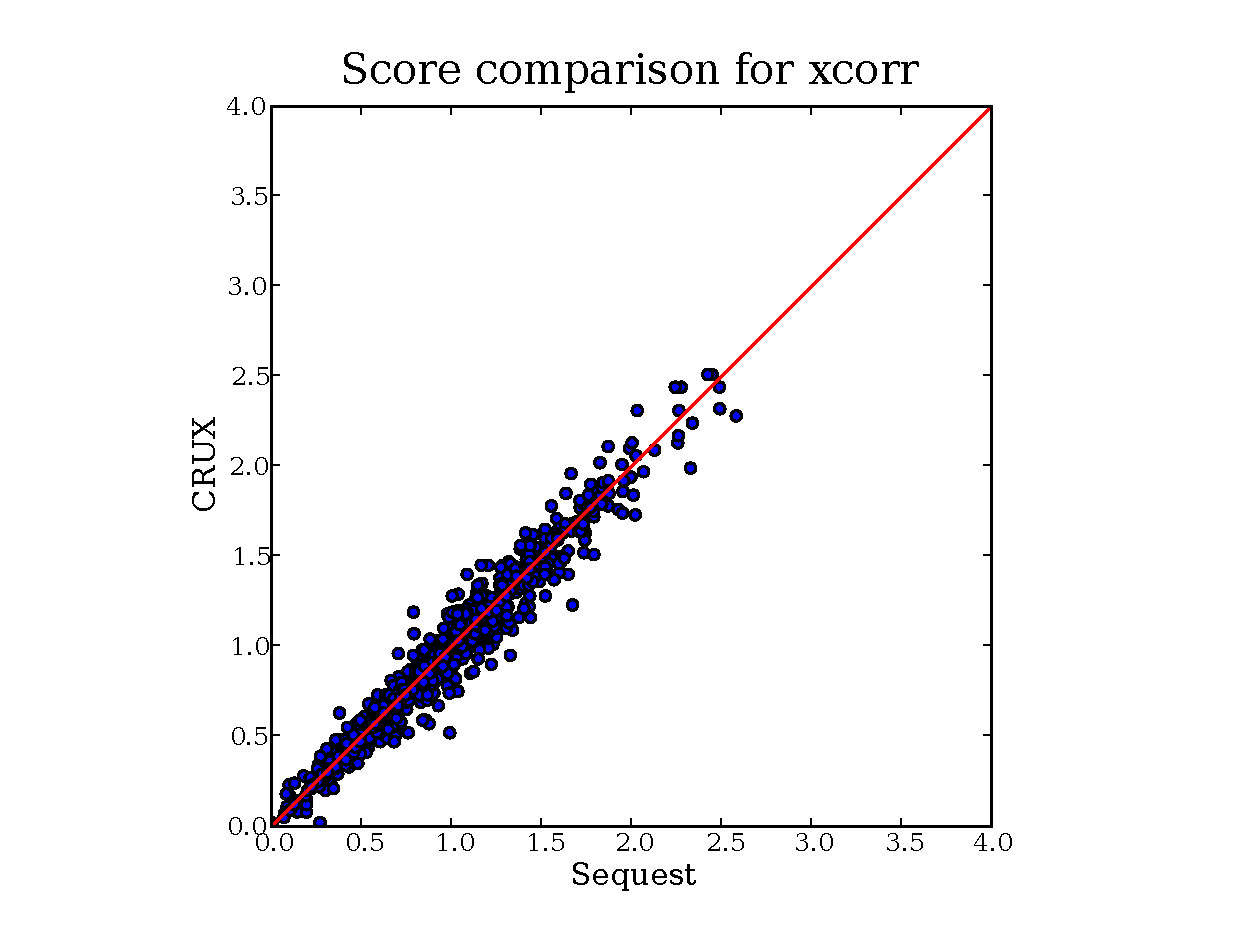
\includegraphics[width=2.5in]{../../results/paper-figure/second-score/fig-2-random-xcorr.eps} \\
  A & B \\
  \end{tabular}
  \caption{{\bf Re-implementation of $Sp$ and $Xcorr$ scoring functions.}
  The figure plots, for a collection of randomly generated spectra and
  randomly associated peptides 
  $Sp$ (A) and $XCorr$ (B) scores as computed by Crux as a function of the
  same scores as computed by {\sc Sequest}. These spectra should cover
  spectra from all possible fragmentation technologies, including
  MALDI-TOF/TOF and QTOF.
  \label{figure:sp-xcorr-random}}
\end{figure*}


\end{document}
